\documentclass[]{article}
\usepackage{lmodern}
\usepackage{amssymb,amsmath}

\usepackage{minted}

\usepackage{dirtytalk}


\usepackage[nameinlink]{cleveref}    

\usepackage{float}

\newfloat{code}{h}{smp}[section]
\floatname{code}{Code sample}

\crefname{code}{code sample}{code samples}
\Crefname{code}{Code sample}{Code samples}


% use upquote if available, for straight quotes in verbatim environments
\IfFileExists{upquote.sty}{\usepackage{upquote}}{}
% use microtype if available
\IfFileExists{microtype.sty}{%
\usepackage{microtype}
\UseMicrotypeSet[protrusion]{basicmath} % disable protrusion for tt fonts
}{}
\usepackage{geometry}
\geometry{%
letterpaper, % a4paper
left=   40 mm,
right=  40 mm,
top=    15 mm,
bottom= 20 mm,
}
\ifxetex
  \usepackage[setpagesize=false, % page size defined by xetex
              unicode=false, % unicode breaks when used with xetex
              xetex]{hyperref}
\else
  \usepackage[unicode=true]{hyperref}
\fi
\usepackage[usenames,dvipsnames]{color}
\hypersetup{breaklinks=true,
            bookmarks=true,
            pdfauthor={Harm Delva},
            pdftitle={Static Analysis of Dynamic Languages},
            colorlinks=true,
            citecolor=blue,
            urlcolor=blue,
            linkcolor=magenta,
            pdfborder={0 0 0}}
\urlstyle{same}  % don't use monospace font for urls
\usepackage{color}
\usepackage{fancyvrb}
\newcommand{\VerbBar}{|}
\newcommand{\VERB}{\Verb[commandchars=\\\{\}]}
\DefineVerbatimEnvironment{Highlighting}{Verbatim}{commandchars=\\\{\}}
% Add ',fontsize=\small' for more characters per line
\newenvironment{Shaded}{}{}
\newcommand{\KeywordTok}[1]{\textcolor[rgb]{0.00,0.44,0.13}{\textbf{#1}}}
\newcommand{\DataTypeTok}[1]{\textcolor[rgb]{0.56,0.13,0.00}{#1}}
\newcommand{\DecValTok}[1]{\textcolor[rgb]{0.25,0.63,0.44}{#1}}
\newcommand{\BaseNTok}[1]{\textcolor[rgb]{0.25,0.63,0.44}{#1}}
\newcommand{\FloatTok}[1]{\textcolor[rgb]{0.25,0.63,0.44}{#1}}
\newcommand{\ConstantTok}[1]{\textcolor[rgb]{0.53,0.00,0.00}{#1}}
\newcommand{\CharTok}[1]{\textcolor[rgb]{0.25,0.44,0.63}{#1}}
\newcommand{\SpecialCharTok}[1]{\textcolor[rgb]{0.25,0.44,0.63}{#1}}
\newcommand{\StringTok}[1]{\textcolor[rgb]{0.25,0.44,0.63}{#1}}
\newcommand{\VerbatimStringTok}[1]{\textcolor[rgb]{0.25,0.44,0.63}{#1}}
\newcommand{\SpecialStringTok}[1]{\textcolor[rgb]{0.73,0.40,0.53}{#1}}
\newcommand{\ImportTok}[1]{#1}
\newcommand{\CommentTok}[1]{\textcolor[rgb]{0.38,0.63,0.69}{\textit{#1}}}
\newcommand{\DocumentationTok}[1]{\textcolor[rgb]{0.73,0.13,0.13}{\textit{#1}}}
\newcommand{\AnnotationTok}[1]{\textcolor[rgb]{0.38,0.63,0.69}{\textbf{\textit{#1}}}}
\newcommand{\CommentVarTok}[1]{\textcolor[rgb]{0.38,0.63,0.69}{\textbf{\textit{#1}}}}
\newcommand{\OtherTok}[1]{\textcolor[rgb]{0.00,0.44,0.13}{#1}}
\newcommand{\FunctionTok}[1]{\textcolor[rgb]{0.02,0.16,0.49}{#1}}
\newcommand{\VariableTok}[1]{\textcolor[rgb]{0.10,0.09,0.49}{#1}}
\newcommand{\ControlFlowTok}[1]{\textcolor[rgb]{0.00,0.44,0.13}{\textbf{#1}}}
\newcommand{\OperatorTok}[1]{\textcolor[rgb]{0.40,0.40,0.40}{#1}}
\newcommand{\BuiltInTok}[1]{#1}
\newcommand{\ExtensionTok}[1]{#1}
\newcommand{\PreprocessorTok}[1]{\textcolor[rgb]{0.74,0.48,0.00}{#1}}
\newcommand{\AttributeTok}[1]{\textcolor[rgb]{0.49,0.56,0.16}{#1}}
\newcommand{\RegionMarkerTok}[1]{#1}
\newcommand{\InformationTok}[1]{\textcolor[rgb]{0.38,0.63,0.69}{\textbf{\textit{#1}}}}
\newcommand{\WarningTok}[1]{\textcolor[rgb]{0.38,0.63,0.69}{\textbf{\textit{#1}}}}
\newcommand{\AlertTok}[1]{\textcolor[rgb]{1.00,0.00,0.00}{\textbf{#1}}}
\newcommand{\ErrorTok}[1]{\textcolor[rgb]{1.00,0.00,0.00}{\textbf{#1}}}
\newcommand{\NormalTok}[1]{#1}

\setlength{\parindent}{0pt}
\setlength{\parskip}{6pt plus 2pt minus 1pt}
\setlength{\emergencystretch}{3em}  % prevent overfull lines
\providecommand{\tightlist}{%
  \setlength{\itemsep}{0pt}\setlength{\parskip}{0pt}}

\title{Static Analysis of Dynamic Languages}
\author{Harm Delva}
\date{}

% Redefines (sub)paragraphs to behave more like sections
\ifx\paragraph\undefined\else
\let\oldparagraph\paragraph
\renewcommand{\paragraph}[1]{\oldparagraph{#1}\mbox{}}
\fi
\ifx\subparagraph\undefined\else
\let\oldsubparagraph\subparagraph
\renewcommand{\subparagraph}[1]{\oldsubparagraph{#1}\mbox{}}
\fi

\usepackage[noend]{algpseudocode}
\usepackage{algorithm}
\usepackage{cleveref}

\usepackage{amsmath} % nice math symbols     

\usepackage{tikz}

\usetikzlibrary{matrix} % for block alignment
\usetikzlibrary{arrows} % for arrow heads
\usetikzlibrary{calc} % for manimulation of coordinates

% TikZ styles for drawing
\tikzstyle{block} = [draw,rectangle,thick,minimum height=2em,minimum width=2em]
\tikzstyle{sum} = [draw,circle,inner sep=0mm,minimum size=2mm]
\tikzstyle{connector} = [->,thick]
\tikzstyle{line} = [thick]
\tikzstyle{branch} = [circle,inner sep=0pt,minimum size=1mm,fill=black,draw=black]
\tikzstyle{guide} = []
\tikzstyle{snakeline} = [connector, decorate, decoration={pre length=0.2cm,
                         post length=0.2cm, snake, amplitude=.4mm,
                         segment length=2mm},thick, magenta, ->]

\renewcommand{\vec}[1]{\ensuremath{\boldsymbol{#1}}} % bold vectors
\def \myneq {\skew{-2}\not =} % \neq alone skews the dash

\usepackage{minted}
\usemintedstyle{manni}
\usepackage{mathtools}
\usetikzlibrary{positioning, calc}
\usepackage{subcaption}
\usepackage{caption}
\usepackage{graphicx}

\usepackage{tcolorbox}
\tcbuselibrary{minted}
\tcbuselibrary{skins}

\definecolor{bg}{HTML}{F0F3F3}


\begin{document}
\tableofcontents

\maketitle

\section{Introduction}\label{introduction}

The university of Ghent has developed the Dodona platform which students
can use to submit solutions to and receive immediate feedback. This
feedback is in large part done through unit testing. This lets the
students know whether or not their solution is correct but doesn't
really help them forward if it's not. To remedy this, there is a visual
debugger included which students can use to step through their program.
This comes with a couple of caveats unfortunately, for example it's
unable to process file IO. More importantly, it can only let the user
scroll through execution states. If an error occurred after a couple of
thousand executed statements, this becomes a very tedious process.

That's just the nature of debugging. Fortunately, there are ways to
avoid this pain altogether. Some programming languages have a strict
compiler to catch obvious mistakes. There are linter tools such as
JSLint and Pylint which emit warnings on error prone patterns. The
Dodona platform uses these tools as well, and relays the warnings to the
students.

The Pylint tool for Python has noticeably helped students avoid
mistakes. Which in turn allowed them to focus more on the actual
assignment and less on learning how to program. The goal of this thesis
is to build on top of that, giving the students even more and even
better feedback. An extensive data-flow analysis can untangle even the
worst spaghetti code, which makes it a prime starting point for further
analysis and feedback.

\section{Literature}\label{literature}

\subsection{Static Analysis}\label{static-analysis}

NASA's source code of the Apollo 11 Guidance Computer was recently
digitized and put on Github. All of it was written in an Assembly
language and the result worked just fine. The C programming language was
made for the Unix operating system so it could run on various CPU
architectures. In essence it's a pretty light abstraction over Assembly,
it doesn't take much pressure off of the programmers. Unix did just fine
as well. One could argue that programmers don't need tools to aid them
-- they seem to know what they're doing.

As the field of research grew, and with it the projects, it started
becoming apparent that programmers can't always rely on themselves. Even
veteran developers occasionally discover a major vulnerability in their
code -- like the Heartbleed vulnerability in OpenSSL. Everyone makes
mistakes but not all mistakes go unnoticed for years in critical code. A
first line of defense against these costly mistakes is a proof of
correctness. NASA's code was reliable because they had formal proofs
that the most critical parts were correct {[}4, 10, 13{]}. Doing this is
not only a massive amount of work, a proof can still be wrong. An
implementation oversight can easily carry over into a proof oversight,
so extra pair of eyes is needed to check all proofs as well.

Functional programming languages are closely related to this method of
provable correctness, while also automating some of checks. Notable
examples of such languages are Haskell and ML. Both have a strong
theoretical foundation and provide the programmer with a strong type
system to make code easier to reason about. This stands in stark
contrast with languages like C. While Haskell was made to facilitate
writing correct code {[}20{]}, C was made to be \emph{close to the
metal} and efficient {[}35{]}. The C compiler doesn't help the
programmer nearly as much as the Haskell compiler. Correctness is
obviously paramount to any computer program, so C's priorities don't
always align with a programmer's.

That's where static analysers come into play. They analyze a program,
either in its source code form or its compiled form, and try to find as
many possible mistakes as possible. These mistakes are often very subtle
and rare, but encountering one can ruin a person's week. Code sample
\ref{smp:shortset} comes from Google's Error Prone Github page and is a
great example of how subtle serious bugs can be.

\begin{code}
  \begin{tcblisting}{listing only, 
  arc=0pt,
  outer arc=0pt, 
  boxrule=0.2pt,
  minted language=java,
  minted style=autumn,
  minted options={},
  colback=bg }
public class ShortSet {
  public static void main (String[] args) {
    Set<Short> s = new HashSet<>();
    for (short i = 0; i < 100; i++) {
      s.add(i);
      s.remove(i - 1);
    }
    System.out.println(s.size());
  }
}
\end{tcblisting}
\caption{Short Set}\label{smp:shortset}
\end{code}

This code seems to be just fine at first glance, but sample
\ref{smp:shortset_f} contains the analysis.

\begin{code}
  \begin{tcblisting}{listing only, 
  arc=0pt,
  outer arc=0pt, 
  boxrule=0.2pt,
  minted language=HTML,
  minted style=autumn,
  minted options={},
  colback=bg }
error: [CollectionIncompatibleType] Argument 'i - 1' should not be 
passed to this method; its type int is not compatible with its 
collection's type argument Short
      s.remove(i - 1);
              ^
\end{tcblisting}
\caption{Analysis of code sample \ref{smp:shortset}} \label{smp:shortset_f}
\end{code}

Subtracting an \texttt{int} from a \texttt{short} resulted in an
\texttt{int}. In this case it won't cause an actual bug yet because both
types use the same hashing function. The JVM originally didn't support
generics, and their implementation is still a bit rough. The
\texttt{remove} method of a \texttt{List} instance doesn't do any type
checks, its argument can be any \texttt{Object} instance. This can
result in calls that never actually remove anything. If that call
happens to only occur in a corner case in the \(1000^{\text{th}}\)
iteration of a loop, this can lead to some very confusing bugs.

\subsubsection{Powerful Languages}\label{powerful-languages}

Every commonly used programming language is Turing complete, so in
theory they should all be equal. This is a misconception that's been
called the Turing tar-pit {[}30{]}. Everything is possible in a Turing
tar-pit, but nothing of interest is easy. Programming languages where
things of interest are perceived to be easy can be considered powerful.
These languages are often the ones with lenient compilers or runtime
environments such as C, Python, Javascript, \ldots{} In other words,
languages that don't get in the way of the programmer too often.

As illustrated in the previous section this may not always be a good
idea as humans tend to glance over subtle details. This makes the need
for additional tools very important for any project that aims to achieve
high reliability. The alternative is long and painful debugging
sessions. At some point these languages no longer make it easy to do
things of interest in.

\paragraph{C}\label{c}

The C programming language has been one of the most popular programming
languages for a couple of decades now. Depending on who you ask, the
best thing about C is either its efficiency or its simplicity, and both
come at a price. Its simplicity is what gives developers the power they
desire. This comes at a cost however; with great power comes great
responsibility.

Let's focus on the other main attraction of C, the efficiency. This
comes at a cost as well and it's a one many people forget about. C's
\emph{raison d'être} isn't making developers feel good about themselves,
it's generating efficient code. It was created to be a thin abstraction
over various assembly languages that were limiting software development
at the time {[}35{]}. Since not all CPU architectures handle a division
by zero the way, the C specification doesn't specify what to do.

\subparagraph{Undefined Behavior}\label{undefined-behavior}

There are a lot of things the language specification doesn't specify a
behavior for, which leads to undefined behavior. Some are well-known,
such as using freed memory. Others catch people by surprise, dividing by
zero in C for example is undefined behavior. The GNU libc website still
claims that \texttt{1/0} yields \texttt{inf} {[}31{]}, even though the
C99 clearly contradicts them {[}11{]}. The C99 standard did introduce
the \texttt{INF} macro, but it doesn't specify which operations should
result in one. Division by zero is still as undefined as it has always
been.

Entire papers have been written on the subject of undefined behavior
{[}23, 26, 37{]}. One striking thing is how recent a lot of these papers
are. Even though the language is over 40 years old, this is still an
active field of research. Compilers are getting more advanced and with
it the optimizations they perform.

Code sample \ref{smp:undef} was part of PostgreSQL {[}23{]}.

\begin{code}
  \begin{tcblisting}{listing only, 
  arc=0pt,
  outer arc=0pt, 
  boxrule=0.2pt,
  minted language=C,
  minted style=autumn,
  minted options={},
  colback=bg }
if (arg2 == 0)
  ereport(ERROR, 
    errcode(ERRCODE_DIVISION_BY_ZERO),
    errmsg("division by zero"));
                    
/* No overflow is possible */
PG_RETURN_INT32((int32) arg1 / arg2);
\end{tcblisting}
\caption{Undefined Behavior}\label{smp:undef}
\end{code}

The \texttt{ereport} function never returns, it does some logging before
calling \texttt{exit}. In the mind of the developer this prevents the
division by zero on the next line. Looking at the code on Github, the
function this sample came from indicates that calling it will return a
\texttt{Datum} struct. The body of the null check does not return
anything, so the compiler concludes that the rest of the function will
also be executed and division by \texttt{arg2} will always get occur.

Division by zero is undefined in C, so the compiler concludes that
\texttt{arg2} won't ever be zero -- it wouldn't get used in a division
otherwise. As a result, the null check gets flagged as dead code, and is
removed entirely.

Code sample \ref{smp:undef_f} contains the fixed code. By adding an
explicit return (in the form a macro), the compiler leaves the null
check intact.

\begin{code}
  \begin{tcblisting}{listing only, 
  arc=0pt,
  outer arc=0pt, 
  boxrule=0.2pt,
  minted language=C,
  minted style=autumn,
  minted options={},
  colback=bg }
if (arg2 == 0)
{
  ereport(ERROR,
      (errcode(ERRCODE_DIVISION_BY_ZERO),
       errmsg("division by zero")));

  /* ensure compiler realizes we mustn't reach the division 
  (gcc bug) */
  PG_RETURN_NULL();
}
\end{tcblisting}
\caption{Fixed Undefined Behavior}\label{smp:undef_f}
\end{code}

Notice how the comment blames a ``gcc bug''. This illustrates how even
experienced developers seem to misunderstand their language of choice.

\subparagraph{Tools}\label{tools}

Not a single other programming language comes close to having as many
external tools as C (and by extension C++). Many developers heavily
depend on these tools in their usual workflow. One of the most
established ones are the ones in Valgrind.

Valgrind is a suite of dynamic analysis tools, the most famous of which
is Memcheck. Memory related bugs are some of the hardest to track down
because most of them are because of undefined behavior. For example,
using a memory location after freeing might not always crash the
program. There's an informal term for bugs like these:
\emph{heisenbugs}. Something might go wrong but when you try to isolate
the cause everything seems to be just fine. Especially since Address
Space Layout Randomization (ASLR) tends to be disabled during debugging
but not during normal execution.

This is where Memcheck comes into play. It analyses the program during
execution and keeps track of what happens to the memory. This way it can
notice memory related bugs such as use-after-free and report them back
to the developer. Unfortunately it's not a perfect solution. There can
be false positives as well as false negatives, and it is quite
incompatible with some libraries such as OpenMPI {[}32{]}.

A lot of companies rely on analysis tools to manage their large C
projects, and when there's demand in a market, the supply will follow.
There's an impressive amount of commercial analysis tools available.
Coverity is one of the most established ones.

Dawson Engler is one of Coverity's co-founders is one of the leading
researchers in the field of static analysis. He also co-authored a great
paper in which he describes how difficult static analysis is in the real
world {[}2{]}. One particularly interesting part of the paper explains
that there's a fundamental misunderstanding of what programming
languages and compilers are. A programming language can exist as an
abstract idea or a piece of paper. While the language a program is
written in is whatever the compiler accepts. In other words, compilation
is not certification. A good first step for a static analysis tool is to
make sure that the input adheres to the specification. They go on to
pose the hypothetical question: ``Guess how receptive they are to fixing
code the ``official'' compiler accepted but the tool rejected with a
parse error?''

Even with a plethora of tools available, C remains an untamed beast.
Some tools like Valgrind are great at what they do but are still
limited. Other tools like Coverity seem to fight stubborn developers as
often as they fight bugs.

\paragraph{Dynamic Languages}\label{dynamic-languages}

Moving on to the topic of this thesis, dynamic languages. According to
Guido Van Rossum, he made Python because he wanted to make a descendant
of ABC that would appeal to Unix/C hackers {[}15{]}. After reading the
previous section some spidey senses should start tingling.

Javascript's situation isn't great either. There are no namespaces, no
modularization system, no classes, no interfaces, no encapsulation,
\ldots{} Eric Lippert, who was on the ECMA committee during the early
days has a Stackoverflow post where he discusses why Javascript is so
ill-fit for static analysis and programming in the large {[}29{]}. Even
though Stackoverflow is a dubious source for any academic work, the
author's experience should make up for it.

Both languages are known as productive languages. Developers don't spend
a lot of time writing boiler plate code or declaring types, they can get
right to the good part. The dynamic nature of the languages even makes
it easy to write generic functions, which makes code reuse easier and
should make the code easier to maintain.

As the following anecdotal examples illustrate, this isn't always the
case. Most people who have used dynamic languages should be able to
confirm that they can misbehave in the spectacular ways. The examples
are supposed to be relatable and bring back memories of frustrating
debugging sessions.

\subparagraph{Classes}\label{classes}

Lots of developers are familiar with class hierarchies and like using
them. There is one glaring difference between how static languages and
dynamic languages handle classes however. In most static languages, the
class definition declares which methods and attributes are defined for
objects of that class. This isn't the case with dynamic languages,
adding a method to an object is as simple as assigning to a callable
object to an attribute.

This is bad news for a static analysers that try to do type inferencing
on dynamic languages. Consider the following problem that occurred while
working on the Dodona platform.

The Ruby builtin \texttt{String} class provides a \texttt{split} that
does the same thing as in most other languages: its argument is some
separator which it uses to cut the \texttt{String} object into an array
of smaller \texttt{String} objects. Calling the \texttt{split} method on
some object returns the same object. Using \texttt{puts} on the object
just shows the same exact String, weird. The documentation says that it
should work. Testing the method in a REPL environment confirms that the
\texttt{split} method should split the \texttt{String}. A few confused
hours later, it turns out the object wasn't a \texttt{String} but an
\texttt{Array}. The Ruby documentation doesn't mention that
\texttt{Array} defines a \texttt{split} method. Googling ``ruby array
split'' refers to the Ruby on Rails documentation. A library silently
declared a method on a builtin type, and \texttt{puts} prints every
element of an \texttt{Array} on a separate line, so it just prints a
single \texttt{String}.

This sort of reckless approach to classes has some serious implications.
Not only does it confuse newcomers, it confuses static analyzers as
well. Due to the lack of type declarations, a logical alternative would
be type inference. But consider the following case, \texttt{split} is
being called on something that's either an \texttt{Array} or a
\texttt{String} at the current stage of inferencing. A regular Ruby
analysis tool might conclude that the object must be a \texttt{String}.
Analyzing Ruby on Rails code would either require the tool to analyze
the entire framework's code first to learn that it adds a \texttt{split}
method to \texttt{Array}, or it might even require a custom analyzer for
Rails altogether.

This is why static analysis of dynamic languages is typically done using
an extensive data-flow analysis {[}16{]}. You don't have to infer the
type of an object if you know where it came from.

\subparagraph{Refactoring}\label{refactoring}

Python's lack of structure makes it hard to work incrementally. At some
point during implementation of the interpreter, line and column
information had to be added to the AST structure. Python's \texttt{ast}
module contains everything one could need to work on Python's AST,
including \texttt{lineno} and \texttt{col\_offset} for seemingly all
classes. With the exception of a few classes, such as
\texttt{generator}. Implementing generators didn't come until much
later, long after the analyser started relying on the existence of
\texttt{lineno} and \texttt{col\_offset} for every node.

Refactoring dynamic languages is a challenge. What if we want to change
the name of a method called \texttt{add} to \texttt{insert}. Can we
replace all occurrences of \texttt{.add} to \texttt{.insert}? That might
change other classes as well. As discussed in the previous section, type
inferencing is non-trivial. Even IDEs that are renowned for their
ability to refactor code, such as the JetBrains IDEs, rely on manual
feedback to filter out the false positives. Reporting false positives is
not always an option however. That's what causes people to question your
tool {[}2{]}.

\subsubsection{NaN}\label{nan}

As an aside, the existence of NaN should be considered error prone as
well. Some languages like Python and Java do a good job at preventing
\texttt{NaN} from entering your program through raising exceptions, but
once they do find their way in you're left at the mercy of the IEEE 754
standard. The most recent version of the standard is IEEE 754-2008 and
was heavily influenced by the ISO C99 standard, which introduced
\texttt{NaN} and \(\inf\) to the C standard.

Since this standard, if one of the function's argument is \texttt{NaN}
but the other arguments already determine the function's value, the
result is no longer \texttt{NaN}. For example, this means that
\texttt{pow(1,\ NaN)} is equal to \texttt{1}. Mathematically this is at
least a bit dubious, \(1^{0/0}\) shouldn't be defined if \(0/0\) isn't
either. The C99 standard introduced various other oddities {[}11{]}.
\(\texttt{pow(-1, }\pm \inf\texttt{)}\) is \texttt{1} because all large
positive floating-point values are even integers. And having a
\texttt{NaN} in the imaginary part of a complex number does not matter
when the value is being cast to a real number, it's apparently possible
for a value to be only slightly undefined.

It has become normal for \texttt{NaN} values to somehow disappear as if
nothing was wrong, leading to some very confusing bugs. Jonathan Peck
ran into the consequences while implementing his own thesis (personal
correspondence). The Theano framework has a function to compute the
gradient of some expression. A \texttt{NaN} found its way into the input
of this function but the result somehow didn't contain a single
\texttt{NaN}, it became seemingly random noise instead. When
implementing something algorithm intensive, any person's first instinct
would be that the algorithm is wrong.

Static analysis should be able to help alleviate this problem. If the
floating-point value that's being used came from a \texttt{sqrt}
function, there should be an \texttt{isNaN} check first. Alternatively,
the Rust programming language tries not to hide the fact that
floating-pointing values can be \texttt{NaN}. Without providing your own
implementation of the \texttt{Ord} trait for the \texttt{f64} type, it's
impossible to order a vector of \texttt{f64} values because comparing
two \texttt{f64} values might be meaningless. It does however provide an
implementation of the \texttt{PartialOrd} trait, which returns an
\texttt{Option\textless{}Ordering\textgreater{}}, which makes it clear
that the result can be \texttt{None}.

\subsubsection{Safe Languages}\label{safe-languages}

Now that it's firmly established that some languages gladly let their
users shoot themselves in the foot, let's look at languages that protect
their users. Most of these languages are functional languages but there
are notable exceptions such as Ada.

\paragraph{Haskell}\label{haskell}

Having strong ties to the lambda calculus {[}20{]}, Haskell is the
archetype of a safe language. Being a pure functional language, all
state in a Haskell program is implicit and by extension there are no
side-effects. One of core concepts of the language is that Haskell code
should be easy to reason about. That's why this language deserves a
section in a thesis about static analysis and data-flow analysis;
Haskell's design makes these things pleasantly simple.

\begin{code}
  \begin{tcblisting}{listing only, 
  arc=0pt,
  outer arc=0pt, 
  boxrule=0.2pt,
  minted language=python,
  minted style=autumn,
  minted options={},
  colback=bg }
def reset(arg):
  arg.attr = None

x = A()
x.attr = 4
y = x

reset(y)

x.attr += 1
\end{tcblisting}
\caption{Aliasing}\label{smp:aliasing}
\end{code}

Consider the Python code in Code sample \ref{smp:aliasing}. Knowing that
\texttt{x} and \texttt{y} are the same is integral to realizing that
\texttt{x.attr\ +=\ 1} will result in a type error, as \texttt{x.attr}
is None since the call to \texttt{reset}. Haskell has no side-effects --
function calls like \texttt{reset(y)} wouldn't be able to change
anything. Additionally, it has no explicit state and thus no assignments
and no aliasing to begin with. This trait can be mimicked in other
languages using the Static Single Assignment (SSA) form where every
variable is immutable. A later section will discuss this form and how it
relates to code analysis.

\paragraph{Rust}\label{rust}

A newer language that favors safety over accessibility is Rust. While it
does have explicit state, Rust also makes the aliasing problem trivially
easy for static analysers. With some exceptions like the reference
counting types, every piece of memory has a single owner in Rust --
which means that by default there's a single way to access any piece of
data. This prevents aliasing problems like the one in sample
\ref{smp:aliasing} because after executing \texttt{y\ =\ x}, \texttt{x}
is no longer a valid identifier -- its data has been moved to
\texttt{y}. On top of that, Rust has explicit mutability. This concept
came from C/C++ where it's good practice to label all immutable things
with \texttt{const}, except that Rust does it the other way around. This
means that unless \texttt{y} was declared to be mutable, the assignment
to \texttt{y.attr} wouldn't compile either.

In languages like Java which heavily advocate encapsulation it's not
uncommon to write something like a
\texttt{List\textless{}Element\textgreater{}\ getElements()} method, so
that other modules can see which data is present. Returning the original
list would mean anybody can change its contents. That's why it's
considered good practice to return a deep copy of the list instead. Deep
copies carry a significant overhead with them, so developers end up
choosing between a safe architecture or an efficient implementation.
Rust lets data be borrowed, so that other modules can see its contents.
The result is a reference which is very similar to a pointer in C, with
the exception that borrowed references carry a lot more type information
with them. For starters, it's possible to borrow something mutably or
immutably. If there is a single mutable borrow to an object, there can't
be any other borrows at the same time. This is a mechanism that's
supposed to avoid unexpected side-effects. Another thing that's part of
a borrow's type is its lifetime. If object A wants to borrow something
from object B, B has to exist at least as long as A. This mechanism
directly prevents all sorts of memory related bugs that occur in C.

Rust is an interesting example of the relationship between languages
(more specifically the compilers) and static analysers. The Rust
compiler enforces a lot of things that the C compiler doesn't but that
the C community has written their own tools for. One might wonder why C
is even still around if Rust seems to be a more complete package. Part
of the answer is that Rust is a very restrictive language which leads to
frustrated developers. Keeping in mind Coverity's paper {[}2{]}, it's a
lot easier to ignore a analyser than it is to fix a compile error.

In fact, this has received the informal label of being an \emph{XY
problem}. If a person knows how to do something using method X, he's
less likely to learn method Y -- even if method Y is clearly the better
choice. Rust has received a lot of criticism from renowned developers
for ridiculous reasons, such as being unable to have two mutable
references to the same object. That's how they'd do it in C, so it must
be the right way. This problem is relevant in this thesis for two
reasons. For starters, static analysis tools run into the same mentality
issues {[}2{]}. More importantly, it shows that it's important to never
pick up bad habits in the first place. The field of application of this
thesis is ultimately helping students learn how to program, before they
even have any bad habits.

\subsubsection{Middle Ground}\label{middle-ground}

It's unrealistic to expect that all programs be rewritten in safe
languages. That doesn't mean that we should abandon all hope of having
reliable programs though. This is why analysis tools have emerged; to
fill the void.

There is a class of static analysers that's particularly interesting,
the linters. What sets them apart from other tools is that they report
error prone patterns rather than actual errors. Preventing bugs is
better than fixing them. One of the most renowned linting tools is
JSLint, its Github page contains the following wisdom {[}33{]}:

\say{The place to express yourself in programming is in the quality of your ideas and
the efficiency of their execution. The role of style in programming is the same
as in literature: It makes for better reading. A great writer doesn't express
herself by putting the spaces before her commas instead of after, or by putting
extra spaces inside her parentheses. A great writer will slavishly conform to
some rules of style, and that in no way constrains her power to express herself
creatively.}

Few developers should find anything anything wrong in that reasoning.
The main point of contention is which rules to follow. Crockford is a
proponent of using certain language features sparsely {[}6{]}. In his
book titled Javascript: The Good Parts he describes which features of
Javascript he deems good (or great and even beautiful) and which parts
should be avoided. The bad parts are everything that lead to error prone
code in his experience, the usual example is the \texttt{switch}
statement. He has given a presentation at Yahoo where he gives more
examples of why JSLint discourages the patterns that it does {[}28{]}.

\subsection{Inspirations}\label{inspirations}

Analysis tools all serve a common purpose but are ultimately still very
diverse. Static and dynamic analysis tools do things very differently
and even within static analysis tools there's a lot of variation.
Linters work mostly syntactical, focusing on speed and immediate
feedback. Other tools like Coverity do a much deeper analysis and
usually run nightly. Another major difference among static analysers is
soundness. Generally speaking, sound analysis tools are based on formal
logic, slower, more comprehensive but more prone to false positives.
Unsound methods seem to coming out on top as most practical languages
are unsound themselves {[}14{]}. Others simply say that it doesn't
matter how you do it, as long as the results are good {[}2{]}.

\subsubsection{Code Smells}\label{code-smells}

\begin{code}
\centering
  \begin{tcblisting}{listing only, 
  arc=0pt,
  outer arc=0pt, 
  boxrule=0.2pt,
  minted language=python,
  minted style=autumn,
  minted options={},
  colback=bg }
x += 1
y += 1
z += 1

x = sqrt(x)
y = sqrt(y)
z = sqrt(z)

u = x - 1
v = y - 1
w = z - 1
\end{tcblisting}
\caption{Duplication}\label{smp:duplication}
\end{code}

More important than how to do the analysis is perhaps what to look for.
Code smells are a taxonomy of indicators that something may not be right
in the code. The term was coined by Kent Beck in a book on refactoring
{[}8{]}. In that book code smells are indicators that some refactoring
might be necessary. Aimed at software architects, they're informal
descriptions of things that may induce technical debt. They're not
actual bugs yet but error prone patterns, the sort of things Linters aim
to detect. One of the code smells ins \emph{cyclomatic complexity},
i.e.~having too many branches or loops. This is something Pylint also
recognizes. What Pylint lacks however is the refactoring aspect of the
code smell. Code smells were meant to be refactored manually by
professional software architects, but in an educational setting you have
to take into account that the students may not be able to refactor it
themselves.

\begin{code}
\centering
  \begin{tcblisting}{listing only, 
  arc=0pt,
  outer arc=0pt, 
  boxrule=0.2pt,
  minted language=python,
  minted style=autumn,
  minted options={},
  colback=bg }
def foo(x):
    x += 1
    x = sqrt(x)
    return x - 1

u = foo(x)
v = foo(y)
w = foo(z)
\end{tcblisting}
\caption{Refactored version of sample \ref{smp:duplication}}\label{smp:duplication_f}
\end{code}

There are also code smells that linters currently do not pick up because
they'd require deep analysis. The most notable of which would be the
\emph{Code Duplication} smell. JetBrains has developed some of the best
refactoring IDEs such as IntelliJ and PyCharm, but started off by
developing code refactoring tools such as IntelliJ Renamer for Java and
Resharper for C\#. Made for commercial code bases, these tools are
ultimately advanced heuristics that still miss obvious duplication.
PyCharm 2016 was unable to find the duplication in code sample
\ref{smp:duplication}. Even it should probably be refactored to
something like code sample \ref{smp:duplication_f}.

\begin{code}
\centering
  \begin{tcblisting}{listing only, 
  arc=0pt,
  outer arc=0pt, 
  boxrule=0.2pt,
  minted language=python,
  minted style=autumn,
  minted options={},
  colback=bg }
x += 1
x = sqrt(x)
u = x - 1

y += 1
y = sqrt(y)
v = y - 1

z += 1
z = sqrt(z)
w = z - 1
\end{tcblisting}
\caption{Alternative order of sample \ref{smp:duplication}}\label{smp:duplication_2}
\end{code}

JetBrain's tools are closed source so it's unclear whether or not
\ref{smp:duplication} was deemed too simple to refactor. Assuming they
work in a similar fashion as competing tools however, it's the order of
statements that causes it to fail. Tools like Simian, Sonar, PMD, and
Dup Loc all work on a token stream in the same order as it appears in
the file. Code sample \ref{smp:duplication_2} illustrates how sample
\ref{smp:duplication} could be reordered so that tools can detect the
duplication just fine.

\begin{code}
\centering
  \begin{tcblisting}{listing only, 
  arc=0pt,
  outer arc=0pt, 
  boxrule=0.2pt,
  minted language=python,
  minted style=autumn,
  minted options={},
  colback=bg }
x = []

s = int(input()) + 1
x.append(s)
s = int(input()) + 1
x.append(s)
s = int(input()) + 1
x.append(s)
s = int(input()) + 1
x.append(s)

\end{tcblisting}
\caption{Duplication}\label{smp:duplication_3}
\end{code}

When analyzing student code, this can be a serious limitation. Consider
code sample \ref{smp:duplication_3}, which just reads 4 numbers from
\texttt{stdin}, increments them, and stores them in \texttt{x}. Even if
this duplication gets detected, most tools are targeted at professional
developers who would never write code like this. The critical difference
is that the refactoring shouldn't introduce a new function but a loop
such as in \ref{smp:duplication_3_f}.

\begin{code}
  \begin{tcblisting}{listing only, 
  arc=0pt,
  outer arc=0pt, 
  boxrule=0.2pt,
  minted language=python,
  minted style=autumn,
  minted options={},
  colback=bg }
x = []

for _ in range(4):
  s = int(input()) + 1
  x.append(s)
\end{tcblisting}
\caption{Refactored version of sample \ref{smp:duplication_3}} \label{smp:duplication_3_f}
\end{code}

Compilers face the same problem; their refactorings are optimizations.
We'll revisit this problem in a later section about the Static Single
Assignment (SSA) form.

There are some other code smells besides code duplication that could be
interesting for new programmers. The following list contains some that
at first glance look like the most promising.

\begin{itemize}
\tightlist
\item
  \emph{Large class}: A class that's grown too large and probably has
  too many responsibilities.
\item
  \emph{Long method}: Much like the previous one, this method probably
  has too many responsibilities.
\item
  \emph{Inappropiate intimacy}: When a class heavily depends on
  implementation details of another class.
\item
  \emph{Excessive use of literals}: Also known as magic numbers, these
  should probably become descriptive constants.
\item
  \emph{Cyclomatic complexity}: Too many branches, also informally
  referred to as \emph{spaghetti code}. Linters do a fair job at
  pointing them out but offer little help in fixing them.
\end{itemize}

\subsubsection{Compilers}\label{compilers}

Static analysers aren't the only tools that aim to make code better --
compilers do so as well. Refactoring from a software architect's point
of view is aimed at making the code easier to read and maintain.
Optimizations are aimed at making code more efficient. These two things
sometimes do completely opposite things, unfolding the loop in
\ref{smp:duplication_3_f} results in sample \ref{smp:duplication_3} for
example. Both operations transform code in a conservative manner though,
i.e.~without changing the semantics (of valid code). Optimization is a
very active area of research, with companies like Google and Apple
working on the LLVM, Oracle on the JVM, Red Hat on the GCC, \ldots{}
More importantly, even the most esoteric features in compilers have
proven their worth as they're part of a real product, which gives
confidence that a static analysis that uses the same principles will
work as well.

\paragraph{SSA}\label{ssa}

Static Single Assignment (SSA) form is a program representation that's
well suited to a large number of compiler optimization such as constant
propagation {[}24{]}, global value numbering {[}1{]}, and code
equivalance detection {[}25{]}. The term was first used in a paper by
IBM {[}1{]} in the 80s but had little practical success initially. It
wasn't until several optimizations were found {[}5, 7{]} that it started
becoming popular. Since then it's found its way into most popular
compilers. LLVM has used it for its virtual instruction set since its
inception in 2002 {[}37{]}, it's what powered Java 6's JIT {[}12{]}, and
it's what's behind recent GCC optimizations {[}17, 18{]}.

The idea is very simple, every variable can only be assigned to once.
This can be done by adding incremental numbers to each variable. For
example, \texttt{x\ =\ x\ +\ 1} becomes
\(\texttt{x}_1 \texttt{ = x}_0 \texttt{ + 1}\). This is a trivial
transformation for straight-line code but becomes a bit harder when
dealing with branches. Figure \ref{fig:ssa} illustrates how to handle
such code. Every branch introduces new variables as before and a
\emph{phi-node} gets inserted at the of the branch. This node mimics a
function call which can return either of its two arguments. This doesn't
correspond to an actual function call, it's just a token that gets
inserted to help with the analysis.

\begin{figure}
    \centering
    \begin{subfigure}[t]{0.44\textwidth}
      \resizebox{\linewidth}{!}{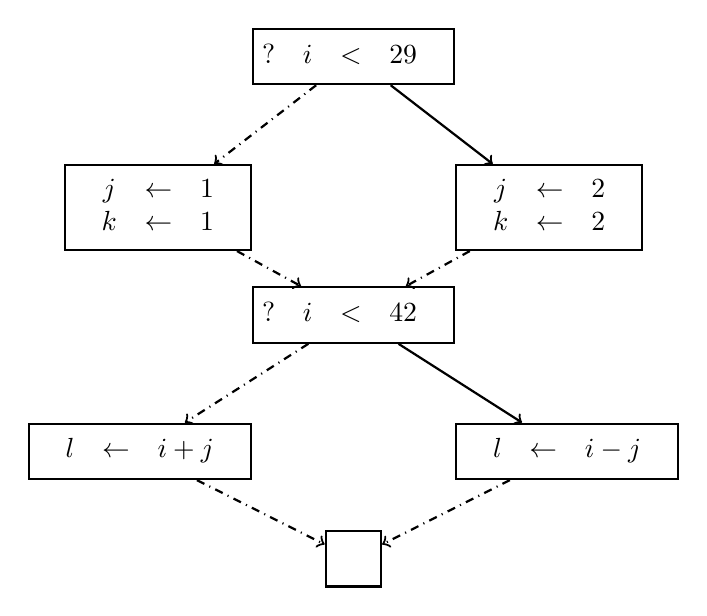
\begin{tikzpicture}
	  \node[block] (base) {$\begin{matrix*}
			? & i &<& 29 &\\
		  \end{matrix*}$
	   }; 
	  
	  \node[block, below left = 1cm and 0cm of base] (neg1) {
	  	$\begin{matrix*}
	  		&j &\gets& 1 &\\
	  		&k &\gets& 1 &
	  	\end{matrix*}$
	  }; 
	  
	  \node[block, below right = 1cm and 0cm of base] (pos1) {
		$\begin{matrix*}
			&j &\gets& 2& \\
			&k &\gets& 2&
		\end{matrix*}$
	  }; \&

	  \node[block, below = of {$(pos1)!0.5!(neg1)$}] (merge1) 		  			  {
	  $\begin{matrix*}
	  ? & i &<& 42 &\\
	  \end{matrix*}$
	  }; \&


	  \node[block, below left = 1cm and 0cm of merge1] (neg2) {
	  $\begin{matrix*}
	  &l &\gets& i + j &\\
	  \end{matrix*}$
	   
	  }; 
	  
	  \node[block, below right = 1cm and 0cm of merge1] (pos2) {
		$\begin{matrix*}
			&l &\gets& i - j &\\
		\end{matrix*}$
		}; 
	  

	  \node[block, below = of {$(pos2)!0.5!(neg2)$}] (merge2) 		  			  {
	  $\begin{matrix*}

	  \end{matrix*}$
	  };

	% now link the nodes

	\draw [connector] (base) --  (pos1);
	\draw [dash dot, connector] (base) --  (neg1);
	\draw [dash dot, connector] (pos1) -- (merge1);
	\draw [dash dot, connector] (neg1) -- (merge1);
	\draw [connector] (merge1) -- (pos2);
	\draw [dash dot, connector] (merge1) -- (neg2);
	\draw [dash dot, connector] (pos2) -- (merge2);
	\draw [dash dot, connector] (neg2) -- (merge2);


  \end{tikzpicture}}
      \caption{Original form}
      \label{fig:ssa_before}
  \end{subfigure}
    \begin{subfigure}[t]{0.55\textwidth}
      \resizebox{\linewidth}{!}{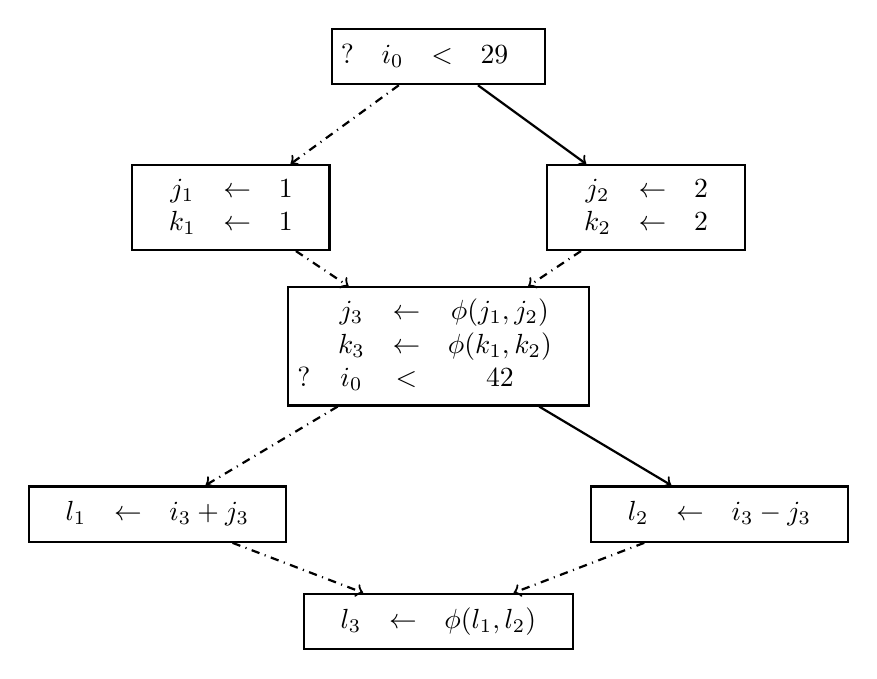
\begin{tikzpicture}
  \node[block] (base) {$\begin{matrix*}
		? & i_0 &<& 29 &\\
	  \end{matrix*}$
   }; 
  
  \node[block, below left = 1cm and 0cm of base] (neg1) {
  	$\begin{matrix*}
  		&j_1 &\gets& 1 &\\
  		&k_1 &\gets& 1 &
  	\end{matrix*}$
  }; 
  
  \node[block, below right = 1cm and 0cm of base] (pos1) {
	$\begin{matrix*}
		&j_2 &\gets& 2& \\
		&k_2 &\gets& 2&
	\end{matrix*}$
  }; \&

  \node[block, below = of {$(pos1)!0.5!(neg1)$}] (merge1) 		  {
  	$\begin{matrix*}
  		&j_3 &\gets& \phi(j_1, j_2)& \\
  		&k_3 &\gets& \phi(k_1, k_2)& \\
  		? & i_0 &<& 42 &\\
  	\end{matrix*}$
  }; \&


  \node[block, below left = 1cm and 0cm of merge1] (neg2) {
  	$\begin{matrix*}
  		&l_1 &\gets& i_3 + j_3 &\\
  	\end{matrix*}$
   
  }; 
  
  \node[block, below right = 1cm and 0cm of merge1] (pos2) {
	$\begin{matrix*}
		&l_2 &\gets& i_3 - j_3 &\\
	\end{matrix*}$
	}; 
  

  \node[block, below = of {$(pos2)!0.5!(neg2)$}] (merge2) 		  {
  	$\begin{matrix*}
		&l_3 &\gets& \phi(l_1, l_2)& \\
  	\end{matrix*}$
  };

% now link the nodes

\draw [connector] (base) --  (pos1);
\draw [dash dot, connector] (base) --  (neg1);
\draw [dash dot, connector] (pos1) -- (merge1);
\draw [dash dot, connector] (neg1) -- (merge1);
\draw [connector] (merge1) -- (pos2);
\draw [dash dot, connector] (merge1) -- (neg2);
\draw [dash dot, connector] (pos2) -- (merge2);
\draw [dash dot, connector] (neg2) -- (merge2);
\end{tikzpicture}}
        \caption{SSA form}
        \label{fig:ssa_after}
    \end{subfigure}
    \caption{SSA transformation}
    \label{fig:ssa}
\end{figure}

\subparagraph{Memory SSA}\label{memory-ssa}

The SSA form has a lot of benefits, as cited in the beginning of this
section, but is limited to scalar values and is not well suited for
structures and arrays. One of the solutions to this problem is Memory
SSA as implemented by GCC {[}17{]}. This is a transformation that runs
on a sufficiently low-level representation of the source code. It has to
be low-level so that there's a notion of \texttt{LOAD} and
\texttt{STORE} instructions.

Because the actual memory locations are not known during compilation
some abstractions are needed. GCC uses compiler symbols which they
called tags to represent regions of memory along with two virtual
operators \texttt{VDEF} and \texttt{VUSE}. For every \texttt{LOAD} a
\texttt{VUSE} of some tag(s) gets inserted, and likewise for
\texttt{STORE} and \texttt{VDEF}.

There are three types of tags:

\begin{itemize}
\tightlist
\item
  \emph{Symbol Memory Tag} (SMT): These are the result of a
  flow-insensitive alias analysis and is almost purely type-based. For
  example, all dereferences of an \texttt{int*} receive the same tag.
\item
  \emph{Name Memory Tag} (NMT): These are the result of a points-to
  analysis applied after the program is in SSA form and inherits its
  flow-sensitive properties {[}17{]}. In other words, multiple SSA forms
  get used.
\item
  \emph{Structure Field Tags} (SFT): These are symbolic names for the
  elements of structures and arrays.
\end{itemize}

Tags get used in a similar way as variables in the regular SSA
algorithm. Assigning to a tag is like assigning to all symbols that have
received that tag. In the original implementation, \emph{call
clobbering}, i.e.~a function call overwrites some memory of an argument,
such as in code sample \ref{smp:aliasing} is handled the same way as
global variables {[}17{]}. Quoting the authors:
\say{All call clobbered objects are grouped in a single set}. The
current implementation has rewritten all call-clobber related code to
use an \emph{aliasing-oracle} {[}27{]}.

LLVM's usage of Memory SSA is not quite as documented. Their
documentation refers to GGC's paper {[}17, 34{]} and mention that
\say{Like GCC’s, LLVM’s MemorySSA is intraprocedural.}. As mentioned in
the previous section, this isn't entirely true for GCC anymore. It
doesn't seem to be true for LLVM either, a recent publication describes
\emph{Static Value-flow} analysis which produces an interprocedural SSA
form {[}22{]}. It has been part of LLVM since 2016 and like GCC's
implementation it uses the results of an external points-to analysis.

\subsubsection{Symbolic Execution}\label{symbolic-execution}

Rather than using concrete values, symbolic execution uses symbolic
values. Those values represent possible values through a set of
constraints. This technique is commonly used to find interesting corner
cases for unit testing {[}3, 19, 21{]} and the original SSA paper used
similar principles as well to make their analysis more precise {[}1{]}.

At each branch point a \emph{path constraint} gets introduced, which is
a symbolic expression that must be true for the current branch to be
taken. If there are no values that satisfy all the constraints, the
branch gets flagged as dead code. In the case of a static analysis tool
this will most likely result in a warning, a compiler will just remove
the dead branch. For example, consider code sample \ref{smp:symb}.
\texttt{y\ \textgreater{}\ 0} becomes a constraint during the execution
of the positive branch, as well as \texttt{x\ \textgreater{}\ -1}. The
former constraint is pretty simple to add, the latter requires some
serious bookkeeping. Symbolic execution is closely related to data-flow
analysis.

\begin{code}
  \begin{tcblisting}{listing only, 
  arc=0pt,
  outer arc=0pt, 
  boxrule=0.2pt,
  minted language=python,
  minted style=autumn,
  minted options={},
  colback=bg }
x = int(input())
y = x + 1

if y > 0:
    z = sqrt(y)
else:
    z = 0
\end{tcblisting}
\caption{Symbolic Execution} \label{smp:symb}
\end{code}

Symbolic execution is a very powerful tool but comes with a few
limitations. One is the \emph{state explosion problem}, the number of
paths can increase \emph{very} fast. The Java Pathfinder manages this
problem using state matching and backtracking {[}19{]}. State matching
will check if a similar state has already been processed, if it has it
will backtrack to the next state that still has unexplored choices.

Another limitation is that symbolic executors typically work on scalar
values. Things get a lot harder when dealing with structures and
collections. Consider code sample \ref{smp:symb2} for example which
defines a function \texttt{foo} that prints \texttt{homogeneous} if and
only if its argument is a collection and all elements in that collection
are of the same type. Not only does the positive branch introduce a
constraint on the length of \texttt{x}, all elements have to be of the
same unspecified type as well. The most advanced symbolic executor for
Python seems to be PyExZ3 but even that one doesn't handle heterogeneous
collections. The relation between uniqueness and the length of a set is
also non-trivial, even though it's a very \emph{pythonic} pattern.

\begin{code}
  \begin{tcblisting}{listing only, 
  arc=0pt,
  outer arc=0pt, 
  boxrule=0.2pt,
  minted language=python,
  minted style=autumn,
  minted options={},
  colback=bg }
def foo(x):
  if len(set(map(type, x))) == 1:
    print('homogeneous')
  else:
    print('heterogeneous')
\end{tcblisting}
\caption{Symbolic Execution Challenge} \label{smp:symb2}
\end{code}

\section{Fosite}\label{fosite}

Named after the Frisian god Fosite and foresight, Fosite is the name of
the abstract interpreter developed for this thesis. A relatively unknown
god, Fosite is the god of reconciliation, justice, and mediation. These
are also qualities that a static analyser should aim to have to gain a
user's trust {[}2{]}.

\subsection{Area of Application}\label{area-of-application}

Unlike most existing tools, Fosite's focus is analysing small student
submissions. This has both advantages and disadvantages. The biggest
advantage is that we're free to explore precise but inefficient methods.
Not entirely free however, since feedback should be fast (\(< 1s\))
because a lot of students will send a lot of submissions at the same
time. Imagine being a stressed out student, working on your final exam
and every submission takes a minute to run because submissions come in
faster than they get processed. It would also be nice if the tool has
little runtime dependencies, since by the Dodona design it'll have to
run in Docker containers. These two requirements make the Rust
programming language a good fit, since it generates fast native code
without the unexpected problems C and C++ might induce.

Perhaps the most requirement of all, any warnings have to be as detailed
as possible. More details should make the errors more convincing and
will be met with less resistance from the user {[}2{]}. This is
important when dealing with new programmers; simply pointing out bad
style is not enough if that person does not know how to fix it
themselves. Fosite uses a data-flow analysis to pinpoint the source of
problems and uses that information to inform the user.

The analysis should work as close as possible to the submitted code and
at the very least maintain a one-to-one relationship to it. This is
important because the end goal is automated refactoring, which becomes
hard when the input becomes mangled beyond recognition.

\subsection{Approach}\label{approach}

As a first step towards automated refactoring, Fosite is an abstract
interpreter with the intention of doing a data-flow analysis. This by
itself isn't entirely new; PyPy uses a similar principle to power their
optimizations {[}36{]}. PyPy's solution is intraprocedural though which
isn't ideal. Others have successfully used abstract interpreters to
perform a may-alias analysis on Python with the goal of optimization
{[}9{]}. Fosite is based on their conclusions and results but is
ultimately made for a different cause, i.e.~detailed static analysis.

The result isn't exactly an SSA form. The Memory SSA approach by the GCC
and LLVM isn't an option since that relies on a low-level
representation. That's a luxury we don't have, we need to stay close to
the original source code. Regular SSA is of course an option since PyPy
does it {[}36{]}, but is limited to intraprocedural analysis.

Fosite generates \emph{use-def} information instead. A \emph{use} refers
to any data dependency, such as resolving a variable name or retrieving
an element from a collection. A \emph{def} is the inverse such as
assigning something to a variable name or inserting an element into a
collection. Within Fosite, a \emph{use} and a \emph{def} are
respectively called a dependency and a change. As with SSA, incremental
numbering can be applied to subsequent changes. The main difference with
regular SSA is that this requires a separate data structure. This allows
a single expression or statement to have multiple changes. For example,
a conditional statement's dependencies and changes are the sum of its
branches'. A conditional statement is exactly that -- a statement, and
it can be useful during refactoring to treat it as a single atomic
thing. Another useful consequence of this is that a function call can
induce multiple changes, for each of its call clobbered arguments.

To achieve the same level of precision as Memory SSA, Fosite uses two
kinds of changes and dependencies. For starters, there's the usual
identifier dependency, which is useful for to model reachability of
data. Consider code sample \ref{smp:dep} in which \texttt{x} gets
defined twice. In between assignments the first value of \texttt{x} gets
used to call in a call to \texttt{print}. This gets modeled using an
identifier dependency. Another sort of dependency is the object
dependency, which is useful to model an internal state dependency. The
second assignment to \texttt{x} assigns a list to it, which gets printed
as well. Before printing however an element gets appended to it.
Appending an element to a list doesn't change anything about the
identifier and thus can't be modeled in the same way. In other words,
the final call to \texttt{print} has a dependency to both the \texttt{x}
identifier and to whichever object \texttt{x} points to at the same time
-- and both dependencies serve their own purpose.

\begin{code}
  \begin{tcblisting}{listing only, 
  arc=0pt,
  outer arc=0pt, 
  boxrule=0.2pt,
  minted language=python,
  minted style=autumn,
  minted options={},
  colback=bg }
x = int(input())
y = int(input())
print(x - y)

x = []
x.append(1)
print(x)
\end{tcblisting}
\caption{Dependency Example} \label{smp:dep}
\end{code}

There are hidden dependencies in this program as well. The first two
lines of code will read two lines from \texttt{stdin} and parse them to
integers. The order in which this happens is important since the two
values get subtracted from each other. This can be modeled by adding
implicit state. The call to \texttt{input} both depends on the implicit
state and changes it, which will ensure that the relative order between
the two calls remains the same. Other IO functionality such as the
\texttt{print} call will do the same. Implicit state can easily be
modeled by designating a specific and hardcoded object to be the
internal state.

\subsection{Modules}\label{modules}

Since languages tend to share a lot of features, it's not unthinkable to
have an abstract interpreter that can process multiple languages. The
first thing this would need is a common input format. Fosite defines a
\emph{General Abstract Syntax Tree} (GAST), which is like other AST
structures with a few exceptions. First of all, it has to be able to
capture all \emph{syntactic} features of the languages it supports; the
semantics aren't important yet. There's a good chance that adding
support for an additional language will require some new nodes or some
extra information in existing nodes. Since only things will have to get
added interpreting the existing languages can just ignore the additional
node types. Another thing that's special about the GAST is that every
node has its unique identifier, and the identifiers are totally ordered.
If one node's identifier is less than another's, that must mean it came
before that other node in the original source file. This is important to
accurately report warning, but also because some optimizations rely on
it.

The GAST only provides a common syntactical framework to work on, the
interpreter has to be able to add semantics to this. A different
\texttt{Executor} instance may be assigned for every supported node for
every supported language. Languages that share the same features can
reuse existing \texttt{Executor} implementations. Common and fundamental
features such as function scoping are even available inside the
interpreter's implementation itself.

\subsection{Power of Interpretation}\label{power-of-interpretation}

While linters recognize error prone patterns, interpreters can recognize
error prone logic as well as some outright errors. An additional benefit
of an interpreter-based approach is that it approaches feedback the same
way a person would: starting at the beginning, step by step. This
section gives a few interesting examples of what an interpreter can do
that linters (or at least PyLint) can't. '

\begin{code}
  \begin{tcblisting}{listing only, 
  arc=0pt,
  outer arc=0pt, 
  boxrule=0.2pt,
  minted language=python,
  minted style=autumn,
  minted options={},
  colback=bg }
def foo():
    for ...:
        for ...:
            if ...:
                return ...
            elif ...:
                return ...
\end{tcblisting}
\caption{Function Returns} \label{smp:return}
\end{code}

Code sample \ref{smp:return} contains an error prone pattern of
Python-like code. A student had written something like this which
resulted in one out of 200 unit tests failing. Written like this, it's
possible that none of the intended \texttt{return} statements get
executed. If this happens the return value is going to be \texttt{None},
which makes the unit test fail in an unexpected way -- nowhere did they
specify a \texttt{None} value should be returned. Fosite gives an
accurate description of the cause -- a \texttt{return} statement was
missing -- instead of just the result.

\begin{code}
  \begin{tcblisting}{listing only, 
  arc=0pt,
  outer arc=0pt, 
  boxrule=0.2pt,
  minted language=python,
  minted style=autumn,
  minted options={},
  colback=bg }
x = []
...
while tuple([0] * i) not in x:
    ...
    x += tuple([0] * i)
\end{tcblisting}
\caption{Heterogeneous Collections} \label{smp:nohomo}
\end{code}

One of the exercises required that a sequence of tuples should be
generated, stopping whenever a tuple of zeroes has been added. Code
sample \ref{smp:nohomo} is based on one of the submissions. Up until the
adding of the tuple of zeroes, the type of \texttt{x} had been
\texttt{List{[}Tuple{[}int{]}{]}} (in the notation used by Python 3.5
type hints). Instead of appending the tuple however, \texttt{+=} will
concatenate the tuple's elements to \texttt{x}. This changes the type to
\texttt{List{[}Union{[}int,\ Tuple{[}int{]}{]}{]}}. This transition to a
heterogeneous collection is valid Python code but ultimately very error
prone. In fact, this causes an infinite loop in this case, as the
expected element never gets added.

\begin{code}
  \begin{tcblisting}{listing only, 
  arc=0pt,
  outer arc=0pt, 
  boxrule=0.2pt,
  minted language=python,
  minted style=autumn,
  minted options={},
  colback=bg }
def change(x, d = None):
  list1 = ''
  list2 = []
  for i in range(0, len(x)):
    while x[i] != ' ':
      list2 += x[i]
    list1 += translate(list2[0], d)
    list2 = []
  return list1
\end{tcblisting}
\caption{Endless Loop} \label{smp:nostop}
\end{code}

Although deciding whether or not any given program will never stop is
impossible, it is possible in some trivial cases. Those trivial cases
also happen to be quite common. Code sample \ref{smp:nostop} is an
excerpt from a submission. The student intended to tokenize the string
\texttt{x}, building the token in \texttt{list2}. Every token should
then get translated and the translated token gets stored in
\texttt{list1}. There are a number of mistakes but the most important
one is arguably the endless \texttt{while} loop. The student wanted
index \texttt{i} to be a starting position of the token, with the
\texttt{while} loop building the token from that point. That's of course
not what the code does, the same character will get added over and over
since none of the values in the loop condition ever change. Data-flow
analysis remembers when and where variables get their values, so it can
be used to recognize that the variables are still the same. This
approach will also flag any \texttt{while\ True} loop as error prone,
which is arguably a good thing.

\subsection{Implementation}\label{implementation}

\subsubsection{Core Objects}\label{core-objects}

\begin{itemize}
\tightlist
\item
  No values at the time, so limited symbolic execution
\item
  Collections do get modeled, but is very hard
\end{itemize}

\paragraph{Pointers and Objects}\label{pointers-and-objects}

\paragraph{Paths and Mappings}\label{paths-and-mappings}

Ordered by node ID, very important

\paragraph{Scope}\label{scope}

Find example of why this is a non-trivial component.

\begin{itemize}
\item
  Introduce Frames
\item
  Every frame corresponds to a branching node in the execution path
\item
  A frame contains its own set of mappings, of all changes that happened
  in this execution path
\item
  Changing an identifier starts at the root
\item
  Iterate over the nodes in the change's path
\item
  If the scope doesn't have enough frames, push new frames corresponding
  to the current node in the iteration
\item
  Only have to check the number of frames, not the actual branches the
  frame corresponds to

  \begin{itemize}
  \tightlist
  \item
    Assuming that the scope's contents are consistent with the current
    execution state two things can happen during assignment
  \item
    The last change to the scope was done in the same execution path. In
    this case, there are enough frames as it is.
  \item
    The scope's execution path is a strict subset of the current
    execution path. In this case, we only have to append the missing
    frames. Ordering of the AST nodes ensures that we know exactly where
    the subset ends.
  \item
    This system depends on the correct merging of frames, see later
  \end{itemize}
\item
  Resolving an identifier starts at the right, the most recent change in
  this scope
\item
  Absolutely no need to introduce branches corresponding to the current
  execution path
\item
  Resolving an identifier does not include the information of the
  frame's path node -- or its parents' path nodes.
\end{itemize}

Code sample \ref{smp:resolution} illustrates why name resolution is done
this way.

\begin{code}
  \begin{tcblisting}{listing only, 
  arc=0pt,
  outer arc=0pt, 
  boxrule=0.2pt,
  minted language=python,
  minted style=autumn,
  minted options={},
  colback=bg }
x = 42
if cond:
  y = 'string'
  x + y
\end{tcblisting}
\caption{Name Resolution}\label{smp:resolution}

\end{code}

This example will always fail if line 4 is reached, because in that case
\texttt{x} will always have type \texttt{int}, while \texttt{y} will
always have type \texttt{string}. So naturally, we want to report it in
the same way.

\begin{itemize}
\tightlist
\item
  Merging frames is a necessary step to ensure consistency the the
  interpreter's execution state.
\item
  Two ways of merging

  \begin{itemize}
  \tightlist
  \item
    Actually merging the last two frames into the parent frame (used for
    function scoping)
  \item
    Discarding the last two frames (used for block scoping)
  \item
    Latter is easy, former requires some special attention
  \end{itemize}
\end{itemize}

As illustrated in code sample \ref{smp:merge}, merging requires some
special attention.

\begin{code}
  \begin{tcblisting}{listing only, 
  arc=0pt,
  outer arc=0pt, 
  boxrule=0.2pt,
  minted language=python,
  minted style=autumn,
  minted options={},
  colback=bg }x = 42
y = 'string'

if cond:
  x = '42'

x + y 
\end{tcblisting}
\caption{Merging}\label{smp:merge}
\end{code}

If the negative branch of the condition at line 4 is not taken, the
above code will fail at line 7. In that case, \texttt{x} still has the
value it received at line 1, but is that all that should be reported?
\texttt{x} only has that value if the negative was taken. So if we want
to accurately describe why it has that value, that information should be
there as well.

This can be achieved by simply resolving the identifiers for both
possible branches, and adding the frame's path node to every result; as
described in algorithm \ref{alg:merge}.

\begin{algorithm}
    \caption{Merge}\label{alg:merge}
    \begin{algorithmic}[1]
        \Function{merge} {}
          \State $\texttt{negative} \gets \texttt{frames.peek()}$
          \State $\texttt{positive} \gets \texttt{frames.peek()}$
          \State $\texttt{parent} \gets \texttt{frames.peek()}$
          \State $\texttt{identifiers} \gets \texttt{positive.identifiers} \cup \texttt{negative.identifiers}$
          \State $\texttt{mappings} \gets []$
          \ForAll{identifiers}
            \State $\texttt{nmap} \gets \texttt{resolve(identifier)}$
            \State $\texttt{nmap.augment(negative.node)}$
            \State $\texttt{mappings += nmap}$
          \EndFor
          \State $\texttt{switch\_ranches()}$
          \ForAll{identifiers}
            \State $\texttt{pmap} \gets \texttt{resolve(identifier)}$
            \State $\texttt{pmap.augment(positive.node)}$
            \State $\texttt{mappings += pmap}$
          \EndFor
          \State $\texttt{parent.add\_mappings(mappings)}$
        \EndFunction
    \end{algorithmic}
\end{algorithm}

\subsubsection{Conditionals}\label{conditionals}

\textbf{Observation}

Every execution branch is either taken, or it isn't. Figuring out which
is the case is well-known to be uncomputable, for the simple reason that
the branch condition can be arbitrarily hard to evaluate. This implies
that in some cases, we can't decide whether or not a given branch gets
taken. The best we can do in these conditions is conclude that the
branch \emph{might} get taken. In the following section, we'll denote
this possibility with \texttt{Maybe}, in line with Python's
\texttt{True} and \texttt{False}.

\textbf{Observation}

In some cases, we do need a definitive answer. Consider the following
examples

\begin{Shaded}
\begin{Highlighting}[]
\ControlFlowTok{if}\NormalTok{ current }\KeywordTok{is} \VariableTok{None}\NormalTok{:}
\NormalTok{  current }\OperatorTok{=}\NormalTok{ datetime.now()}
\end{Highlighting}
\end{Shaded}

\begin{Shaded}
\begin{Highlighting}[]
\ControlFlowTok{if}\NormalTok{ current }\KeywordTok{is} \KeywordTok{not} \VariableTok{None}\NormalTok{:}
  \BuiltInTok{print}\NormalTok{(}\StringTok{'}\SpecialCharTok{\{\}}\StringTok{-}\SpecialCharTok{\{\}}\StringTok{'}\NormalTok{.}\BuiltInTok{format}\NormalTok{(current.year, }
\NormalTok{                       current.month))}
\end{Highlighting}
\end{Shaded}

The above examples gives a pretty good indication that in some cases, we
really need an exact example. This is particularly important for any
sort of input validation. The first example is a common pattern for
filling in optional arguments, while the second one is just good
practice in general. Other examples include checking the length of a
certain collections and type-checks.

\textbf{Boolean Expressions with Certainty}

There aren't a lot of boolean expressions which we can evaluate with
certainty. Luckily enough, the ones that we can do are mostly the ones
of interest. The \texttt{is} operator for example should compare the
addresses of two objects and return \texttt{True} if and only if they're
equal. So internally, we can mimic this behavior -- and answer with
certainty and under which conditions, the objects have the same address
in our own analysis. The other possibilities are harder to do, and the
best we can realistically return is \texttt{Maybe}.

The \texttt{==} operator is a special case. If the \texttt{\_\_eq\_\_}
method was implemented correctly, this should at the very least return
\texttt{True} if the two objects being compared are the same -- as with
\texttt{is}. The analyzer in its current state does not properly support
analysis of operator overloading, so it will assume that
\texttt{\_\_eq\_\_} does indeed have a sane implementation. The analysis
of the \texttt{==} operator in this case becomes the same as the
analysis of the \texttt{is} operator. Likewise for the
\texttt{\textless{}=} and \texttt{\textgreater{}=} operators.

The \texttt{and} and \texttt{or} operators are quite obvious.
\texttt{and} will return \texttt{True} if both sides are true with
certainty, \texttt{False} if either side is false with certainty, and
\texttt{Maybe} in any other case. The \texttt{or} operator is analogous.

\textbf{Definition: containment}

A path \(A\) is contained in another path \(B\) if every node of path
\(A\) occurs in the same way as it does in path \(B\)

\subsubsection{Path exclusion}\label{path-exclusion}

When executing an execution branch, we should have information about why
that specific branch is being executed. If that information includes for
example that we are sure that \texttt{x} is not \texttt{None}, we should
disregard any mapping that says the opposite. And even better, we can
exclude any mapping that would occur under the same contradictory
conditions -- even if those mappings don't have an explicit connection
to \texttt{x}. For example in the following trivial example:

\begin{Shaded}
\begin{Highlighting}[]
\ControlFlowTok{if}\NormalTok{ cond1:}
\NormalTok{  y }\OperatorTok{=} \VariableTok{None}
\NormalTok{  z }\OperatorTok{=} \VariableTok{None}
  
\ControlFlowTok{if}\NormalTok{ y }\KeywordTok{is} \KeywordTok{not} \VariableTok{None}\NormalTok{:}
  \BuiltInTok{print}\NormalTok{(z.attribute)}
\end{Highlighting}
\end{Shaded}

In the positive branch of the first condition, there's a point where
both \texttt{y} and \texttt{z} become \texttt{None}. After evaluating
the second branching condition, we can be absolutely sure that the
positive branch of the second branch will not be taken if the positive
branch of the taken has been taken. In effect, this means that the
mapping for \texttt{z} where it receives the value \texttt{None}in the
first branch is of no use while evaluating \texttt{z.attribute}.

The exclusion of certain mappings is what we'll conveniently call
\emph{path exclusion}. We can give this term a more formal
representation as well.

Assume that resolving an identifier \(x\) resulted in a set of mappings
\(M\). Every mapping \(m \in M\) is of the form \((p, a)\), where \(a\)
is the address to which \(x\) can point, and \(p\) is the execution path
that's required to get this mapping from \(x\) to \(a\).

Call \(R\) the set of restrictions; the set of every execution pth that
is of no concern while evaluating. If there exists a path \(r\) in \(R\)
for a given mapping \((p, a)\), for which it holds that \(p\) is
contained within \(r\), we can exclude the mapping from the current
evaluation.

\section{Results}\label{results}

\section{Discussion}\label{discussion}

\section{Future Work}\label{future-work}

\section*{References}\label{references}
\addcontentsline{toc}{section}{References}

\hypertarget{refs}{}
\hypertarget{ref-equality}{}
{[}1{]} Alpern, B. et al. 1988. Detecting Equality of Variables in
Programs. \emph{Conference Record of the 15th Annual Symposium on
Principles of Programming Languages} (1988), 1--11.

\hypertarget{ref-coverity}{}
{[}2{]} Bessey, A. et al. 2010. A few billion lines of code later: Using
static analysis to find bugs in the real world. \emph{Commun. ACM}. 53,
2 (Feb. 2010), 66--75.

\hypertarget{ref-symb3}{}
{[}3{]} Cadar, C. et al. 2008. KLEE: Unassisted and automatic generation
of high-coverage tests for complex systems programs. \emph{Proceedings
of the 8th usenix conference on operating systems design and
implementation} (Berkeley, CA, USA, 2008), 209--224.

\hypertarget{ref-nasa2}{}
{[}4{]} Carey and Sturm \emph{Space software}.

\hypertarget{ref-dominance}{}
{[}5{]} Cooper, K.D. et al. 2001. A simple, fast dominance algorithm.
\emph{Software Practice \& Experience}. (2001).

\hypertarget{ref-goodparts}{}
{[}6{]} Crockford, D. 2008. \emph{JavaScript: The good parts}. O'Reilly
Media, Inc.

\hypertarget{ref-increment}{}
{[}7{]} Cytron, R. et al. 1991. Efficiently computing static single
assignment form and the control dependence graph. \emph{ACM Trans.
Program. Lang. Syst.} 13, 4 (Oct. 1991), 451--490.

\hypertarget{ref-refactor}{}
{[}8{]} Fowler, M. 1999. \emph{Refactoring: Improving the design of
existing code}. Addison-Wesley Longman Publishing Co., Inc.

\hypertarget{ref-interpret}{}
{[}9{]} Gorbovitski, M. et al. 2010. Alias analysis for optimization of
dynamic languages. \emph{Proceedings of the 6th symposium on dynamic
languages} (New York, NY, USA, 2010), 27--42.

\hypertarget{ref-nasa3}{}
{[}10{]} Hand, J.A. 1971. \emph{Guidance, navigation and control}. MIT.

\hypertarget{ref-C99}{}
{[}11{]} ISO/IEC 2003. Rationale for international standard--
programming languages-- c.

\hypertarget{ref-hotspot}{}
{[}12{]} Kotzmann, T. et al. 2008. Design of the java hotspot\&Trade;
client compiler for java 6. \emph{ACM Trans. Archit. Code Optim.} 5, 1
(May 2008), 7:1--7:32.

\hypertarget{ref-nasa1}{}
{[}13{]} Kreide, H. and Lambert, D.W. 1964. \emph{Computation: Aerospace
computers in aircraft, missiles, and spacecraft}.

\hypertarget{ref-unsound}{}
{[}14{]} Livshits, B. et al. 2015. In defense of soundiness: A
manifesto. \emph{Commun. ACM}. 58, 2 (Jan. 2015), 44--46.

\hypertarget{ref-lutz}{}
{[}15{]} Lutz, M. 1996. \emph{Programming python}. O'Reilly \&
Associates, Inc.

\hypertarget{ref-madsen}{}
{[}16{]} Madsen, M. 2015. \emph{Static analysis of dynamic languages}.
Aarhus University.

\hypertarget{ref-memoryssa}{}
{[}17{]} Novillo, D. 2007. Memory ssa-a unified approach for sparsely
representing memory operations. \emph{Proc of the gcc developers'
summit} (2007).

\hypertarget{ref-treessa}{}
{[}18{]} Novillo, D. 2003. Tree ssa a new optimization infrastructure
for gcc. \emph{In proceedings of the 2003 gcc developers} (2003),
181--194.

\hypertarget{ref-symb2}{}
{[}19{]} Păsăreanu, C.S. and Rungta, N. 2010. Symbolic pathfinder:
Symbolic execution of java bytecode. \emph{Proceedings of the ieee/acm
international conference on automated software engineering} (New York,
NY, USA, 2010), 179--180.

\hypertarget{ref-haskell}{}
{[}20{]}, Paul Hudak et al. 2007. A history of haskell: Being lazy with
class. (June 2007).

\hypertarget{ref-symb1}{}
{[}21{]} Rhodes, D. et al. 2014. Dynamic detection of object capability
violations through model checking. \emph{SIGPLAN Not.} 50, 2 (Oct.
2014), 103--112.

\hypertarget{ref-svf}{}
{[}22{]} Sui, Y. and Xue, J. 2016. SVF: Interprocedural static
value-flow analysis in llvm. \emph{Proceedings of the 25th international
conference on compiler construction} (New York, NY, USA, 2016),
265--266.

\hypertarget{ref-wang}{}
{[}23{]} Wang, X. et al. 2012. Undefined behavior: What happened to my
code? \emph{Proceedings of the asia-pacific workshop on systems} (New
York, NY, USA, 2012), 9:1--9:7.

\hypertarget{ref-constant}{}
{[}24{]} Wegman, M.N. and Zadeck, F.K. 1991. Constant propagation with
conditional branches. \emph{ACM Trans. Program. Lang. Syst.} 13, 2 (Apr.
1991), 181--210.

\hypertarget{ref-equivalent}{}
{[}25{]} Yang, W. et al. 1989. \emph{Detecting program components with
equivalent behaviors}.

\hypertarget{ref-guide}{}
{[}26{]} A guide to undefined behavior in c and c++.
\url{http://blog.regehr.org/archives/213}.

\hypertarget{ref-oracle}{}
{[}27{]} Alias improvements branch.
\url{https://gcc.gnu.org/wiki/Alias_Improvements}.

\hypertarget{ref-crockford}{}
{[}28{]} Crockford on javascript - section 8: Programming style \& your
brain. \url{https://www.youtube.com/watch?v=taaEzHI9xyY}.

\hypertarget{ref-lippert}{}
{[}29{]} Dynamic languages make for harder to maintain large codebases.
\url{http://softwareengineering.stackexchange.com/a/221658}.

\hypertarget{ref-tarpit}{}
{[}30{]} Epigrams on programming.
\url{http://www-pu.informatik.uni-tuebingen.de/users/klaeren/epigrams.html}.

\hypertarget{ref-gnu}{}
{[}31{]} Infinity and nan.
\url{http://www.gnu.org/software/libc/manual/html_node/Infinity-and-NaN.html}.

\hypertarget{ref-mpi}{}
{[}32{]} Is open mpi 'valgrind-clean' or how can i identify real errors?
\href{https://www.open-mpi.org/faq/?category=debugging\#valgrind_clean\%0A}{https://www.open-mpi.org/faq/?category=debugging\#valgrind\_clean
}.

\hypertarget{ref-jslint}{}
{[}33{]} JSLint. \url{https://github.com/douglascrockford/JSLint}.

\hypertarget{ref-memoryssallvm}{}
{[}34{]} MemorySSA. \url{http://llvm.org/docs/MemorySSA.html}.

\hypertarget{ref-cdev}{}
{[}35{]} The development of the c language.
\url{https://www.bell-labs.com/usr/dmr/www/chist.html}.

\hypertarget{ref-pypy}{}
{[}36{]} The rpython toolchain.
\url{http://rpython.readthedocs.io/en/latest/translation.html\#flow-graphs}.

\hypertarget{ref-lattner}{}
{[}37{]} What every c programmer should know about undefined behavior.
\url{http://blog.llvm.org/2011/05/what-every-c-programmer-should-know.html}.

\end{document}